% This is the main file for the template for the coursework during
% PhD studies at the University of Zagreb, Faculty of Electrical Engineering
% and Computing in Zagreb, Croatia
% Initial version: February 2018

% Author: Marijo Simunovic 

% search apt-cache search name.sty

%%%%%%%%%%%%%%%%%%%%%%%%%%%%%%%%%%%%% SETTINGS %%%%%%%%%%%%%%%%%%%%%%%%%%%%%%%%
\documentclass[12pt,oneside, a4paper]{article}
\usepackage[pdftex]{graphicx}
\graphicspath{ {images/} } %place all images here
\usepackage[bf, font=small]{caption} %image caption settings
\usepackage[labelfont=small, font=small]{subcaption}
\usepackage{csvsimple} % requires texlive-latex-extra
\usepackage[toc,page]{appendix}

\usepackage{amsmath}
\numberwithin{equation}{section}
\usepackage{relsize}
\usepackage[hidelinks]{hyperref} %clickable references without borders

\usepackage[T1]{fontenc}
\usepackage[utf8]{inputenc}
\usepackage[croatian]{babel} % requires texlive-lang-european package
\usepackage{color}

\usepackage[left=2.5cm,right=2.5cm,top=2.5cm,bottom=2.5cm]{geometry}
\usepackage{lmodern} % allows arbitrary font size
\linespread{1.3} % this is one-and-a-half spacing
%paragraph settings 
%\setlength{\parskip}{1em}
\setlength{\parindent}{2em}

\usepackage[square, numbers, sort]{natbib} 
% change the name of Bibliography heading into "Literatura"
\addto\captionscroatian{%
  \renewcommand{\bibname}{Literatura}
}
\addto\captionscroatian{%
  \renewcommand{\appendixname}{Dodatak}
}
%\usepackage{titlesec} %chapter name manipulation
%% remove chapter name and number
%\titleformat{\chapter}[display]
%   {\normalfont\bfseries}{}{0pt}{\Huge}
%

%narrow underscore
\renewcommand{\_}{\textscale{.7}{\textunderscore}}

\usepackage[dvipsnames]{xcolor}
\usepackage{fancyvrb}
% redefine \VerbatimInput
\RecustomVerbatimCommand{\VerbatimInput}{VerbatimInput}%
{fontsize=\footnotesize,
%
frame=lines,  % top and bottom rule only
framesep=2em, % separation between frame and text
rulecolor=\color{Gray},
%
label=\fbox{\color{Black}data.txt},
labelposition=topline,
%
commandchars=\|\(\), % escape character and argument delimiters for
                       % commands within the verbatim
commentchar=*        % comment character
}


\begin{document}

%%%%%%%%%%%%%%% PRVA UNUTARNJA STRANICA / FIRST INNER PAGE %%%%%%%%%%%%%%%%
\begin{titlepage}
  \fontsize{16pt}{20pt}\selectfont
  \fontfamily{phv}\fontseries{mc}\selectfont
  \newgeometry{left=3cm,right=3cm,top=3cm,bottom=2.5cm}
  \setlength{\intextsep}{0pt plus 0pt minus 0pt}

  \begin{center}
    \begin{figure}[ht!]
      \begin{center}
        
\includegraphics[height=4.1184cm, width=5.94cm]{logo_unizg2}
      \end{center}
    \end{figure}		
    \vspace{0cm}
    {FAKULTET ELEKTROTEHNIKE I RAČUNARSTVA} \\
    \vspace{3cm}
    Marijo Šimunović \\
    \vspace{2cm}
    {\fontsize{22pt}{22pt}\selectfont\textbf{Detekcija intronskih i egzonskih sekvenci u molekuli DNK upotrebom stabala odlučivanja}} \\
    \vspace{2cm}    
    SEMINARSKI RAD \\
    \vspace{5cm}    % adjust this spacing if necessary
    \vfill{Zagreb, 2018.}
  \end{center}
  \restoregeometry
\end{titlepage}

\tableofcontents
%%%%%%%%%%%%%%%%%%%%%%%%%%%%%%%%% LOF %%%%%%%%%%%%%%%%%%%%%%%%%%%%%%%%%%%%%%%%%
\clearpage
\listoffigures
\clearpage % start new page
%%%%%%%%%%%%%%%%%%%%%%%%%%%%%%%%% LOT %%%%%%%%%%%%%%%%%%%%%%%%%%%%%%%%%%%%%%%%%
% insert optional list of tables
\listoftables
%\section{Abstrakt}
%Ako treba sazetak

\clearpage
\chapter{Uvod}
\label{ch:intro}


\clearpage
\chapter{Poglavlje 1}
\label{ch:ch1}


\clearpage
\section{Opis razvojnog okruženja za dubinsku analizu}
\label{ch:ch2}

\subsection{Programski alati za dubinsku analizu}
Za obradu i preprocesiranje skupa podataka korišten je programski jezik \textit{Python} (verzija 3.5)
u kombinaciji sa bibliotekama \textit{pandas}, \textit{sklearn} te \textit{matplotlib} i \textit{seaborn} za grafički prikaz rezultata.
\textit{pandas} je biblioteka otvorenog koda koja implementira brze i fleksibilne strukture podataka kako bi se korisniku omogućilo što lakše i intuitivnije upravljanje podacima\cite{McKinney01}. Ova biblioteka omogućuje korištenje različitih tipova podataka
\begin{itemize}
   \item Tabularni podaci sa stupcima heterogenog tipa (kao u SQL ili Excel tablicama)
   \item Uređeni i neuređeni skupovi vremenskih podataka
   \item Proizvoljni podaci u matričnom obliku s oznakama redova i stupaca
   \item Bilo kakav drugi oblik statističkih skupova podataka koji ne mora nužno biti označen
\end{itemize}

\textit{scikit-learn} je biblioteka otvorenog koda i sadrži skup algoritama za strojno učenje i dubinsku analizu podataka\cite{Pedregosa01}. Obuhvaća širok spektar funkcionalnosti, od preprocesiranja podataka preko učenja različitih modela do evaluacije dobivenih rezultata.
Skripta za obradu podataka napisana je u razvojnom okruženju \textit{Jupyter Notebook} i dostupna je u \textit{GitHub}\footnote{\url{https://github.com/AntiCodeOn/Misc/tree/main/DataMining/GenomeSplice}} repozitoriju. Dubinska analiza provedena je korištenjem programskog alata Weka\cite{Weka01}.

\subsection{Skup podataka za dubinsku analizu}

Skup podataka nad kojim je napravljena dubinska analiza potječe iz banke genoma
(Genbank 61.1) i može se preuzeti sa repozitorija za strojno učenje UCI\footnote
{\url{https://archive.ics.uci.edu/ml/datasets/Molecular+Biology+(Splice-junction+Gene+Sequences)}}
u komprimiranoj datoteci. Skup sadrži 3190 instanci sa 63 atributa.
Prvi atribut u tablici je klasa. Podaci pripadaju jednoj od tri kategorije:
\begin{itemize}
   \item "IE" - slijed u genomu koji se nalazi na granici intron egzon
   \item "EI" - slijed u genomu koji se nalazi na granici egzon intron
   \item "N" - slijed u genomu za koji je poznato da ne sadrži granicu između egzona i introna
\end{itemize}
Drugi atribut je tekstualni identifikator instance.
Preostali atributi su zapravo sekvenca šezdeset slova koje označavaju nukleotide
ciljanog mjesta na genomu. U ovom radu se na pozicije pojedinačnih nukleotidnih baza (slova) referiramo pozitivnim indeksima {1, 2, ..., 60}.
Nukleotidi u skupu podataka su označeni na način prikazan Tablicom \ref{tab:oznake}.

\begin{table}[!ht]
   \caption[Oznake nukleotida u skupu podataka za dubinsku analizu]{
   \textbf{Oznake nukleotida u skupu podataka za dubinsku analizu.} \textit{A, G, C i T se koriste ako se na
   toj lokaciji pojavljuje isključivo jedna od četiri baze. Ukoliko se na istom indeksu u sekvenci
   pojavljuju različite baze, uz sve ostale pozicije s jednakim nukleotidima koristimo oznake D, N, S i R.}}
   \centering
   \begin{tabular}{||c | c ||}
   \hline
   Oznaka atributa & Nukleotid \\ [0.5ex]
   \hline\hline
   A & Adenin \\
   T & Timin \\ 
   G & Guanin \\ 
   C & Citozin \\
   D & Adenin ili Guanin ili Timin \\
   N & Adenin ili Guanin ili Citozin ili Timin \\
   S & Citozin ili Guanin \\
   R & Adenin ili Guanin \\ [1ex]
   \hline
   \end{tabular}
   \label{tab:oznake}
\end{table}


\clearpage
\section{Predobrada podataka i izbor atributa}
\label{ch:ch3}

\subsection{Predobrada}
Za predobradu podataka korišten je programski jezik Python u kombinaciji sa paketom Pandas. Datoteka s podacima \textit{splice\_orig.csv} je učitana u Pandas DataFrame objekt te su dodani nazivi atributa: \textit{class}, \textit{id} i \textit{dna} (vidi Tablicu \ref{tab:dataorig}).
\begin{table}[!ht]
   \caption[Primjeri instanci iz originalnog podataka]{
   \textbf{Primjeri instanci iz skupa podataka za dubinsku analizu} \textit{}}
   \centering
   \begin{tabular}{||c | c | c ||}
   \hline
   class & id & dna \\ [0.5ex]
   \hline\hline
   EI & ATRINS-DONOR-905 & AGACCCGCCGGGAGGCGGAGGACCTGC... \\
   EI & BABAPOE-DONOR-30 & GAGGTGAAGGACGTCCTTCCCCAGGAG... \\
   EI & CHPIGECA-DONOR-378 & CAGACTGGGTGGACAACAAAACCTTCA... \\
   .. & .. & .. \\
   N & ORAHBG2F-NEG-181  & ATCAATAAGCTCCTAGTCCAGACGCCAT... \\
   N & ORARGIT-NEG-241 & TCTCGGGGGCGGCCGGCGCGGCGGGG... \\
   N & TARHBD-NEG-1981  & AGGCTGCCTATCAGAAGGTGGTGGCTG... \\ [1ex]
   \hline
   \end{tabular}
   \label{tab:dataorig}
\end{table}

Nakon što smo izbacili stupac \textit{id} i podijelili stupac \textit{dna} podaci imaju oblik kao u tablici \ref{tab:datasplit}.

\begin{table}[!ht]
   \caption[Primjeri instanci iz procesiranog skupa podataka]{
   \textbf{Primjeri instanci iz procesiranog skupa skupa podataka za dubinsku analizu} \textit{
Stupac \textit{id} je jedinstveni identifikator vrste za svaki red u tablici i zbog toga ga ne koristimo u analizi podataka. Stupac \textit{DNA} dijelimo na šezdeset stupaca, za svaki nukleotid u DNA nizu po jedan novi stupac, naziva dna\_x gdje x označava indeks nukleotida u originalnom nizu.
   }}
   \centering
   \begin{tabular}{||c | c | c |c | c | c | c ||}
   \hline
   class & dna{\_1} & dna{\_}2 & dna{\_}3\ & dna{\_}4\ & dna{\_}5 & ...\\ [0.5ex]
   \hline\hline
   EI & A & G & A & C & C & ... \\
   EI & G & A & G & G & T & ... \\
   EI & C & A & G & A & C & ... \\
   .. & .. & .. & .. & .. & .. & ... \\
   N & A  & T & C & A & A & ... \\
   N & T  & C & T & C & G & ... \\
   N & A  & G & G & C & T & ... \\ [1ex]
   \hline
   \end{tabular}
   \label{tab:datasplit}
\end{table}

\begin{table}[!ht]
   \caption[Udjeli nukleotida u skupu podataka za dubinsku analizu]{
   \textbf{Udjeli nukleotida u skupu podataka za dubinsku analizu.} \textit{A, G, C i T čine značajnu većinu u skupu podataka. D, N, S i R čine neznatan dio skupa.}}
   \centering
   \begin{tabular}{||c | c | c ||}
   \hline
   Oznaka atributa & Broj atributa & Udio atributa (\%) \\ [0.5ex]
   \hline\hline
   A & 44475 & 23.244 \\
   T & 46298 & 24.196 \\
   G & 50226 & 26.249 \\
   C & 50281 & 26.278 \\
   D & 2  & 0.0010 \\
   N & 56 & 0.0293 \\
   S & 1  & 0.0005 \\
   R & 1  & 0.0005 \\ [1ex]
   \hline
   \end{tabular}
   \label{tab:udjeli}
\end{table}
Tablica \ref{tab:udjeli} pokazuje razdiobu jedinstvenih oznaka nukleotida. Vidimo da vrlo mali udio ima oznaku D, N, S ili R (ukupno 15 redaka). Zbog toga možemo izbaciti ove retke bez značajnog smanjenja skupa podataka za dubinsku analizu. S druge strane, na ovaj način sprječavamo da algoritam da previše važnosti podacima koji spadaju u ovu marginalnu skupinu (eng. \textit{outliers}). 
Jedna od instanci iz klase EI\footnote{HUMALPI1-DONOR} ima nukleotidni niz\textit{ 
ACACAGGGCACCCCCTCANNNNNNNNNNNNNNNNNNNNNNNNNNNNNNNNNNNNNNNNN
}. Čak 42 baze označene su s oznakom N. Ako bi svaki N zamijenili s jednom od četiri moguće baze dobili bismo 4\textsuperscript{42} kombinacija. Bez provjere u postojećim bazama podataka ne možemo znati koje su od tih kombinacija uistinu dijelovi donorskih sekcija u genomu. Korištenjem ovih kombinacija značajno bismo utjecali na distribuciju skupa podataka jer većina lokacija u genomima nije ni donorska ni akceptorska sekcija gena. 
Ovako obrađen skup podatak spremljen je u datoteku \textit{splice\_filtered.csv}

\subsection{Organizacija podataka atributa}

Prije nego krenemo s procesom obrade podataka dijelimo skup na dva dijela: skup za trening i skup za testiranje. Za testiranje izdvajamo 20\% od ukupnog skupa podataka i njih koristimo samo za završnu ocjenu odabranih trening algoritama. Funkcija \textit{test{\_}train{\_}split} iz modula model{\_}selection. Želimo osigurati da su podaci stratificirani, odnosno da su razdiobe podataka jednake u ishodišnom skupu podataka kao i generiranim skupovima. 
\begin{center}
   \begin{figure}[ht!]
      \begin{center}
         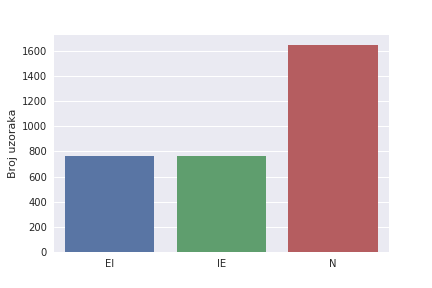
\includegraphics[height=6cm, width=9cm]{dataset_class_dist}
         \caption[Distribucija instanci u skupu podataka]
         {\textbf{Distribucija instanci u skupu podataka po klasama.}\textit{Prevladava klasa N, odnosno nizovi koji ne pripadaju ni akceptorskim ni donorskim nizovima nukleotida. U pojedinačnom genomu ova razlika je još izraženija\cite{Brown01} i kada bismo htjeli koristiti ovaj algoritam na drugim skupovima podataka morali bismo prilagoditi broj instanci odgovarajućim omjerima.}}
         \label{fig:dist_orig}
      \end{center}
   \end{figure}
\end{center}

Metoda \textit{test{\_}train{\_}split} ima argument \textit{stratify} kojem predajemo stupac s klasama. Slike \ref{fig:dist_orig} i \ref{fig:dist_train_test} potvrđuju da su podaci pravilno podijeljeni.

\begin{center}
   \begin{figure}[ht!]
   \begin{subfigure}{.5\textwidth}
         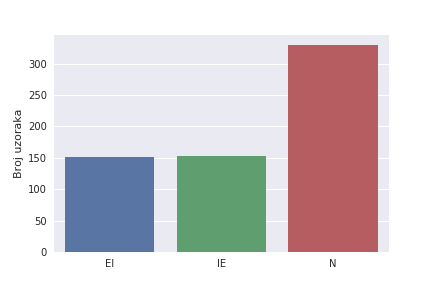
\includegraphics[height=5cm, width=8cm]{testset_class_dist}
         \caption{Trening}
         \label{fig:dist_train}
   \end{subfigure}
   \begin{subfigure}{.5\textwidth}
         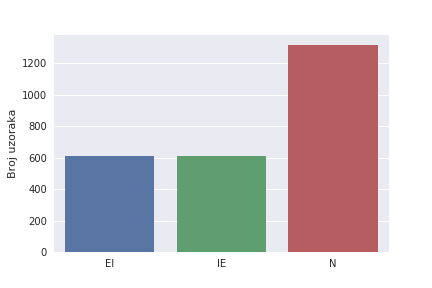
\includegraphics[height=5cm, width=8cm]{trainset_class_dist}
         \caption{Test}
         \label{fig:dist_test}
   \end{subfigure}
   \caption[Distribucija instanci u trening i testnom skupu podataka]
   {\textbf{Distribucija instanci u podijeljenim skupovima podataka po klasama.}\textit{Vidimo da je distribucija skupa za trening (a) i skupa za testiranje (b) jednaka distribuciji izvornog skupa podataka. Razlika je samo ukupnom broju instanci u pojedinome skupu.}}
    \label{fig:dist_train_test}
   \end{figure}
\end{center}

\subsection{Odabir atributa}
Pri kreiranju modela za dubinsku analizu podataka obično nije nužno koristiti sve dostupne atribute skupa podataka. U odabiru najboljih atributa za model primjenjuju se različite tehnike koje se u grubo mogu svrstati u tri kategorije. Metode \textbf{filtriranja} koriste najčešće različite statističke testove kako bi se odredila korelacija\footnote{termin korelacija ovdje koristimo u širem smislu, ne isključivo u statističkom kontekstu} između atributa i izlazne varijable (klase). Druga kategorija, metode\textbf{omotača}\footnote{eng. \textit{wrapper methods}} koriste se podskup atributa nad kojim treniraju model. Na osnovu zaključaka iz ovog modela, dodaju se ili oduzimaju određeni atributi - problem odabira atributa svodi se na problem pretraživanja. \textbf{Ugradbene} metode\footnote{eng. \textit{embedded methods}} kombiniraju kvalitete filterskih i metoda omotavanja korištenjem algoritama koji imaju vlastite ugrađene metode selekcije atributa.

Algoritam stabla odlučivanja ima prirodno ugrađen mehanizam za odabir atributa. Najprije se u postupku konstrukcije rangiraju atributi, a zatim se u postupku podrezivanja smanjuje ukupan broj atributa. Neki računalni znanstvenici\cite{Grabczewski01} zbog ovih karakteristika koriste stablo odlučivanja kao algoritam za odabir atributa koji će se zatim koristiti u drugom modelu (klasifikacija iili regresijski postupak). Budući da je procedura izgradnje stabla odlučivanja poprilično brza onda je moguće i koristiti sve atribute. Međutim, kako bi provjerili ovu hipotezu, kreirat ćemo i dodatne varijante stabla odlučivanja, nad podskupom atributa.

Budući da su svi podaci u skupu nominalni, te da imamo veliki broj atributa, moguće ih je prikazati samo indirektnom mjerom ili parcijalno (Slika\ref{fig:class_dna_x}).
\begin{center}
   \begin{figure}[ht!]
   \begin{subfigure}{.5\textwidth}
         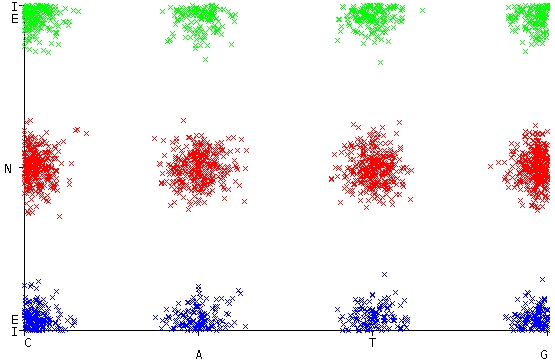
\includegraphics[height=5cm, width=8cm]{class_dna_2}
         \caption{dna{\_}2}
         \label{fig:class_dna_2}
   \end{subfigure}
   \begin{subfigure}{.5\textwidth}
         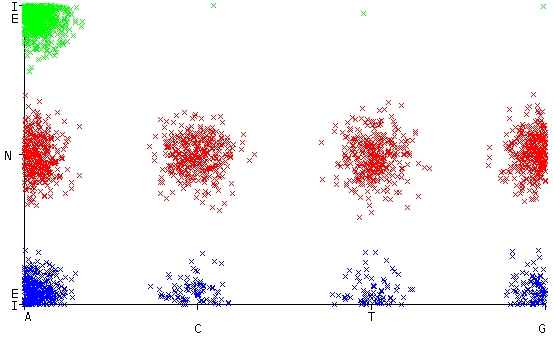
\includegraphics[height=5cm, width=8cm]{class_dna_29}
         \caption{dna{\_}29}
         \label{fig:class_dna_29}
   \end{subfigure}
   \begin{subfigure}{.5\textwidth}
         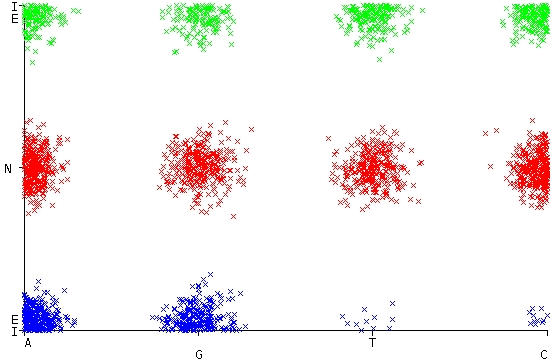
\includegraphics[height=5cm, width=8cm]{class_dna_33}
         \caption{dna{\_}33}
         \label{fig:class_dna_33}
   \end{subfigure}
   \begin{subfigure}{.5\textwidth}
         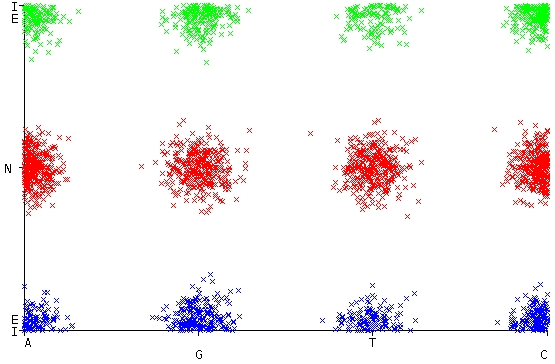
\includegraphics[height=5cm, width=8cm]{class_dna_54}
         \caption{dna{\_}54}
         \label{fig:class_dna_54}
   \end{subfigure}
   \caption[Dijagram rasipanja vrijednosti atributa po klasama]
   {\textbf{Frekvencija vrijednosti atributa po klasama.}\textit{ Distribucija vrijednosti atributa uniformna je na indeksima udaljenima od sredine nukleotidnog niza (\ref{fig:class_dna_2} i \ref{fig:class_dna_54}). Za indekse neposredno prije granice (\ref{fig:class_dna_29}) i poslije granice (\ref{fig:class_dna_33}) donorsko-akceptorskog područja vidimo da postoje izražena koncentracija određenih vrijednosti baza.}}
    \label{fig:class_dna_x}
   \end{figure}
\end{center}
Ovakva razdioba upućuje na zaključak da nisu svi atributi jednako značajni. Zbog toga provodimo postupak selekcije atributa korištenjem prikladnog statističkog testa. Budući da smo već utvrdili da postoji određena frekvencijska relacija vrijednosti atributa i klasa kao logičan postupak nameće se tzv. Hi-kvadrat test.
\subsubsection{Hi-Kvadrat test}
Hi-Kvadrat je test nezavisnosti koji se koristi kako bi se odredilo postoji li značajna veza između dvije nominalne (kategorične) varijable. Frekvencija svake vrijednosti jedne nominalne varijable (atributa) uspoređuje se sa kategorijama druge nominalne varijable (klase). Računaju se očekivane vrijednosti frekvencija vrijednosti atributa i uspoređuju sa stvarnim vrijednostima iz skupa podataka. Podaci se prikazuju u kontigencijskim tablicama. Primjer je dan tablicom \ref{tab:contig}.
\begin{center}
    \begin{table}[!ht]
    \caption[Kontigencijska tablica]{
    \label{tab:contig}
    \textbf{Primjer kontigencijske tablice.} \textit{Stupci su kategorije jedne varijable (atributa), a redovi kategorije druge varijable (klase). Krajnji redak i stupac predstavljaju sumu vrijednosti iznad, odnosno lijevo. Na osnovu sumarnih vrijednosti računaju se očekivane vrijednosti kategorija.}}
   \centering
   \begin{tabular}{||c | c | c | c ||}
   \hline
     & Atr1 & ... & AtrN \\ [0.5ex]
   \hline\hline
   Klasa1 & $O_{11}$ & ... & $O_{1N}$  \\
   ..     & ...    & $O_{mn}$ & ...  \\
   KlasaM & $O_{M1}$ & ... & $O_{MN}$  \\ [1ex]
    \hline
    \end{tabular}
    \end{table}
\end{center}
Najprije se računaju očekivane vrijednosti na osnovu tablice kontigencije korištenjem sljedeće formule

\begin{equation}\label{eq:chiexpect}
E_{ij} = \frac{\sum_{k=1}^{N}O_{ik}\sum_{k=1}^{M}O_{kj}}{N}
\end{equation}

gdje je 

\begin{itemize}
    \item $\sum_{k=1}^{N}O_{ik}$ - suma i-tog retka u kontigencijskoj tablici
    \item $\sum_{k=1}^{M}O_{kj}$ - suma j-tog stupca u kontigencijskoj tablici
    \item N - ukupan broj instanci u skupu podataka.
\end{itemize}

Nakon izračuna očekivanih vrijednosti, možemo se pristupiti izračunu vrijednosti Hi-kvadrat testa neovisnosti na slijedeći način:

\begin{equation}
    \chi^2 = \sum_{i=1}^{M}\sum_{j=1}^{N}\frac{(O_{ij}-E_{ij})^2}{E_{ij}}
\end{equation}

Hi-kvadrat testira određenu hipotezu čiju istinitost pretpostavljamo. Nulta hipoteza pretpostavlja da ne postoji statistički značajna veze između dvije varijable. Alternative hipoteza, pojednostavljeno, pretpostavlja suprotno od nulte hipoteze.

Tablica \ref{tab:chi2} prikazuje primjer kontigencijske tablice za dva atributa, dna{\_2} i dna{\_}29, iz podataka nad kojima vršimo analizu. Odgovarajuća nulta i alternativna hipoteza mogu biti:
\begin{itemize}
    \item $H_0$: Nukleotid na n-tom indeksu nije povezan s klasom nukleotidnog niza, i 
    \item $H_1$: Nukleotid na n-tom indeksu povezan je s klasom nukleotidnog niza.
\end{itemize}

\begin{table}
\centering
    \caption[Sumarni podaci vrijednosti atributa za hi-kvadrat test]{\textbf{Sumarni podaci vrijednosti atributa za hi-kvadrat test.} \textit{Tablični pregled vrijednosti koje se koriste u hi-kvadrat testu za odabir atributa. Za atribut na indeksu 2 vidimo da se broj nukleotidnih baza poklapa sa distribucijom klasa u skupu. Za atribut na indeksu 29 vidimo da vrijednosti značajno odstupaju od razdiobe klasa.}}
    \label{tab:chi2}
    \csvautotabular{"data/chi2table.csv"}
\end{table}
Koristeći \eqref{eq:chiexpect} možemo izračunati da očekivana vrijednost kategorije T za atribut dna{\_}2 u slučaju klase IE iznosi $E_{IE2T} = 756*765/3174 = 182$ i razlika u odnosnu na stvarnu vrijednost je samo 14. U slučaju za atribut dna{\_}29 očekivana vrijednost na istoj poziciji u tablici iznosi $E_{IE29T} = 514*765/3174 = 124$, odnosno razlika je čak 123.

\subsubsection*{Weka chiSquaredAttributeEval}
Kako ne bismo morali ručno raditi izračun Hi-kvadrat vrijednosti cijelog seta koristimo modul \textit{chiSquaredAttributeEval} za selekciju atributa unutar Weka programskog alata. Ovaj paket je dodatni i treba ga naknadno instalirati korištenjem izbornika \textit{Tools->Package Manager} u početnom pregledniku programa.


\clearpage
\section{Stabla odlučivanja}
\label{ch:ch4}

Stabla odlučivanja vrlo su popularna metoda dubinske analize podataka zbog svoje jednostavnosti i brzine. Algoritam koristi “podijeli-pa-vladaj” paradigmu i najjednostavnije se može opisati u rekurzivnom obliku. Najprije se odabire atribut koji će biti korijen stabla. Za svaku moguću vrijednost koju taj atribut može imati izvodi se jedna grana. Na ovaj način se skup podataka dijeli u podskupove. Ako jedan od čvorova stabla dobivenih na ovaj način sadrži samo instance jedne klase, zaustavlja se rekurzivni postupak. Inače, nastavljamo dijeliti preostale podskupove prema novim atributima. Odabir atributa nije proizvoljan, želimo odabrati atribute na takav način da stablo bude što manje tako da naš algoritam radi brže. 

Indukcijski zadatak provodi se nad skupom objekata koji su opisani kolekcijom atributa. Svaki atribut mjeri neko važno svojstvo objekta te u pravilu poprima veličinu iz diskretnog skupa vrijednosti. Objekti pripadaju jednoj od dvije ili više međusobno isključivih klasa. Iz skupa podataka za trening u kojem su klase objekata poznate izvode se klasifikacijska pravila. Ukoliko su atributi adekvatni (objekti s istim vrijednostima atributa pripadaju istoj klasi) uvijek je moguće konstruirati stablo odlučivanja koje će ispravno klasificirati sve objekte u trening skupu\cite{Witten01}. 
Međutim, stablo odlučivanja koje ispravno klasificira samo trening skup nije korisno jer zapravo samo izražava podatke koje imamo u tablici (trening skupa) u obliku stabla. Kako bi se  konstruirano stablo moglo primjeniti i na buduće, dotad neviđene podatke (testni skup) stablo odlučivanja mora sadržavati smislene informacije o odnosima atributa objekta i klase tog objekta. 

Računalni znanstvenik John Ross Quinlan dao je značajan doprinos razvoju algoritama za dubinsku analizu temeljenim na stablima odlučivanja\cite{Quinlan01},\cite{Quinlan02},\cite{Wu01}. Istraživanje je potaknuto potrebom da se unaprijede algoritmi sa sposobnošću pronalaska znanja u samim skupovima podataka bez korištenja domenskih eksperata. Prvi iz niza varijanti stabla odlučivanja koje je dizajnirao, ID3, je dizajniran za skupove podataka s velikim brojem objekata i velikim brojem atributa objekta poštujući ograničenje da konstruirano stablo odlučivanja bude jednostavno (kako bi se ubrzao proces generiranja takvog stabla uz minimalne računalne resurse). Posljedica ovakvih ograničenja u dizajnu je da ID3 ne garantira globalno optimalno stablo odlučivanja\cite{Quinlan02}.

\subsection{C4.5 algoritam}

C4.5 je nasljednik algoritma ID3. Kao i prethodni, C4.5 generira klasifikator u obliku stabla odlučivanja, ali može 
kreirati i klasifikator u razumljivijem formatu, u obliku skupa pravila. Pretpostavimo da postoji skup \textit{S} 
slučajeva. C4.5 konstruira stablo na sljedeći način:
\begin{itemize}
   \item Ako svi slučajevi u \textit{S} pripadaju istoj klasi ili je skup mal, stablo je samo čvor s oznakom najčešće klase u skupu \textit{S}
   \item Inače, odabrati test na jednom atributu s dva ili više ishoda i postaviti ovaj test u korijen stabla s granom za svaki ishod. Podijeliti skup \textit{S} na podskupove \textit{S1}, \textit{S2}, ... ovisno o ishodu svakog test te nastaviti s procedurom rekurzivno za svaki podskup.
\end{itemize}
Ova definicija je poprilično općenita jer bi mogli odabrati mnogo različitih testova. C4.5 koristi dvije heuristike za rangiranje testova
\begin{itemize}
   \item \textit{Informacijska vrijednost IG\footnote{eng. \textit{Information Gain}}}  - minimizira ukupnu entropiju podskupova i
   \item \textit{Omjer dobiti GR\footnote{eng. \textit{Gain Ratio}}} - dijeli IG sa informacijom iz ishoda testa.
\end{itemize}

Dozvoljeni su i numerički i nominalni atributi. Numberički atributi u pravilu koriste testove s pragovima, te ishodi
ovise o tome jesu li vrijednosti atributa veće ili manje (ili jednake) od praga. Kod atributa s diskretnim vrijednostima
u pravilu testovi imaju jednak broj ishoda kao i broj mogućih vrijednosti tog atributa, ali je moguće i grupiranje 
vrijednosti kako bi se smanjio broj ishoda testa, a samim time i složenost konstruiranog stabla.

Inicijalno konstruirano stablo je podložno pretreniranju (eng. \textit{overfitting}) zbog čega se koristi algoritam podrezivanja stabla. Podrezivanje se odvija od listova prema korijenu. Računa se pesimistična procjena učestalosti pogrešak korištenjem binomne razdiobe za slučaj kada je registrirano E događaja, koji ne pripadaju najčešćoj klasi, u N pokušaja, s korisnički definiranim intervalom pouzdanosti. Za podstablo se sumira procjena pogreške svih grana i uspoređuje sa greškom u slučaju da se cijelo podstablo zamjeni čvorom. Ukoliko potonja greška nije veća stablo se podrezuje. Također, moguće je zamjenjivanje podstabla samo jednom njegovom granom ukoliko to ne povećava pogreške\cite{Wu01}.

\subsubsection{Informacijska vrijednost i omjer dobiti}
Algoritam C4.5 koristi osnovne postulate informacijske teorije u procesu izgradnje stabla. Prema teoriji informacije, informacija sadržana u poruci ovisi o vjerojatnosti te poruke $p$ i može se mjeriti u bitovima kao negativan logaritam te vjerojatnosti \cite{Shannon01}. Pretpostavimo da postoji skup instanci $S$ veličine $|S|$ unutar kojeg svaka od instanca pripada točno jednoj od $J$ klasa gdje ukupan broj instanci klase $j$ u skupu $S$ označavamo sa $|C_{jS}|$. Ako nasumično izaberemo jednu instancu iz skupa vjerojatnost da ona pripada klasi $j\in{1,..,J}$ iznosi\begin{equation}
p = \frac{|C_jS|}{|S|}.
\end{equation}
Očekivana informacija takve poruke u odnosu na pripadnost klasi izražena je sumom svih klasa u proporciji sa njihovim udjelima u skupu $S$. 

\begin{equation}
info(S) = -\mathlarger{\sum}_{j}\frac{|C_{jS}|}{|S|}\cdot\log_{2}\frac{|C_{jS}|}{|S|}
\end{equation}
U trening skupu $info(S)$ mjeri prosječnu informaciju potrebnu da bi se identificirala klasa instance iz skupa S. Nakon što smo podijelili skup $S$ u $n$ particija u ovisnosti od ishoda testa $X$ očekivanu informaciju računamo kao težinsku sumu podskupova
\begin{equation}
info_{X}(S) = -\mathlarger{\sum}_{i}\frac{|S_{i}|}{|S|}\cdot info(S_{i})
\end{equation}
Konačno, informacijsku dobit računamo kao
\begin{equation}
gain(X) = info(S)-info_{X}(S)
\end{equation}
U algoritmu ID3 favorizirani su testovi s puno ishoda. Na primjer, u našem testnom skupu atribut \textit{id} je jedinstven za svaku instancu. Korištenjem takvog atributa dobili bismo veliki broj podskupova od kojih svakih sadrži jedan slučaj sa. Budući da bi ovi podskupovi imali samo jednu klasu, $info_{X}S$ bi uvijek bio 0, odnosno iformacijska vrijednost od korištenja ovakvog atributa bi bila maksimalna. Međutim, ovakvo stablo ne bi moglo klasificirati ni jednu novu instancu (jer bi ona imala $id$ koji se nije nalazio u skupu za trening). To je zapravo razlog zašto smo izbacili ovaj atribut u procesu predobrade. C4.5 je popravio ovaj nedostatak korištenjem normalizacije. Izraz
\begin{equation}
split info(X) = -\mathlarger{\sum}_{i}^{n}\frac{|S_{i}|}{|S|}\cdot\log_{2}\frac{|S_{i}|}{|S|}
\end{equation}
predstavlja potencijalnu informaciju dobivenu dijeljenjem skupa $S$ u $n$ podskupova. Ova veličina povezana je s informacijskim sadržajem ishoda testa u usporedbi sa informacijom klasifikacije kao što je u slučaju informacijske dobiti.
\begin{equation}
\label{eq:gr}
GR(X) = info(S)/split info(X)
\end{equation}
Omjer dobiti \ref{eq:gr} izračava udio informacije generiran podjelom nastalom korištenjem testa X \cite{Quinlan02}.

\subsubsection{Nedostatci C4.5 algoritma}
Postoje dva glavna razloga koja utječu na lošije performanse algoritma: ograničenje jednostruke pokrivenosti i fragmentacija. Ograničenje jednostruke pokrivenosti uzrokovano je heurističkom prirodom metode. Konstrukcija C4.5 stabala odvija se tako da se odabire atribut koji je najdiskriminatorniji u cijelom skupu podataka te se na osnovu njega podaci dijele u nepreklapajuće podskupove koji bi trebali imati što više uzoraka iste klase. Svaka podgrupa odgovara jednom pravilu i svaka instanca zadovoljava ograničenja samo jednog pravila (instanca se ne može nalaziti u više podgrupa odjednom). S druge strane, to znači da svaka instanca mora zadovoljiti samo jedno pravilo što rezultira generiranjem manjeg broja značajnih pravila čak i u višedimenzionalnim skupovima podataka. Mali broj značajnih pravila može uzrokovati pristranost u predikcijama. Fragmentacija nastaje zbog generiranje mnogih lokalno važnih, ali globalno nevažnih pravila u podskupovima dublje u stablu \cite{Li01}.


\clearpage
\section{Rezultati analize}
\label{ch:ch5}


Za procjenu uspješnosti klasifikacije koriste se različite mjere. Za razumijevanje rezultata potrebno je razumjeti i problem koji se modelom opisuje i pokusava rjesiti.Klasifikator koji bi uvijek davao klasu N (nije detektirana granica IE ili EI) bi i dalje imao veliku točnost, budući da je većina genoma sastavljena od nekodirajućih dijelova.

\begin{itemize}
   \item Točnost 
   \item TPR
   \item FPR
   \item F-mjera
   \item AUC
   \item ROC
\end{itemize}


Tablica prikazuje uspješnost algoritama korištenjem gore opisanih mjera.


\clearpage
\section*{Zaključak}
\label{ch:conc}
\addcontentsline{toc}{section}{Zaključak}

Razvijeni model pokazuje kako stabla odlučivanja omogućuju kreiranje vrlo uspješnih modela s vrlo malo ili nimalo domenskoga znanja. Sami algoritam u sebi ima heuristiku koja mu omogućuje rangiranje atributa po važnosti te odbacivanja manje važnih atributa. Također, pokazano je da selekcija atributa može imati različite efekte na konačne rezultate, od zadržavanja točnosti uz smanjenje veličine stabla, povećanja točnosti uz zadržanu veličinu stabla do degradacije performansi modela (ista točnost, ali povećano stablo odlučivanja). To je samo još jedna potvrda činjenice da put do najboljeg modela u dubinskoj analizi nije pravocrtan nego podrazumijeva iterativni proces uz postupno podešavanje parametara modela.

Stabla odlučivanja su se za ovaj model pokazala kao vrlo brz i uspješan algoritam i potvrdila pretpostavku da heuristike ugrađene u dizajn modela mogu izabrati kvalitetan podskup podataka. Iako je jedan od najstarijih algoritama u domeni, stabla odlučivanja u različitim varijantama ostaju privlačna zbog svoje jednostavnosti i mogućnosti da generiraju rezultate koji pomažu istražiteljima interpretirati svojstva skupova podataka koji se analiziraju što je zapravo i krajnji cilj svake dubinske analize.


\clearpage
\section*{Dodatak A - Weka modeli za odabir parametara}
\label{ch:addA}
\addcontentsline{toc}{section}{Dodatak A}

\textbf{Izbor atributa korištenjem Hi-kvadrat testa}

\VerbatimInput{chi2attributes.txt}

\textbf{Izbor atributa korištenjem višeslojnog perceptrona}

\VerbatimInput{mpattributes.txt}

%%%%%%%%%%%%%%%%%%%%%%%%%%%% BIBLIOGRAPHY %%%%%%%%%%%%%%%%%%%%%%%%%%%%%%%%%%%%%
% bibliography style file is modified IEEEtran.bst file,
% changed to suit FER's literature style
\clearpage % start new page
\addcontentsline{toc}{section}{Literatura}
\bibliographystyle{IEEEtranFER} 
\bibliography{eg_biblio}

%%%%%%%%%%%%%%%%%%%%%%%%%%%%%%%%% INDEX %%%%%%%%%%%%%%%%%%%%%%%%%%%%%%%%%%%%%%%
% optional index
%\printindex

\end{document}
